% Copyright (C) 2010,2011,2012,2013,2014,2015,2016 The ESPResSo project
% Copyright (C) 2002,2003,2004,2005,2006,2007,2008,2009,2010 
%   Max-Planck-Institute for Polymer Research, Theory Group
%  
% This file is part of ESPResSo.
%   
% ESPResSo is free software: you can redistribute it and/or modify it
% under the terms of the GNU General Public License as published by the
% Free Software Foundation, either version 3 of the License, or (at your
% option) any later version.
%  
% ESPResSo is distributed in the hope that it will be useful, but
% WITHOUT ANY WARRANTY; without even the implied warranty of
% MERCHANTABILITY or FITNESS FOR A PARTICULAR PURPOSE.  See the GNU
% General Public License for more details.
%  
% You should have received a copy of the GNU General Public License
% along with this program.  If not, see <http://www.gnu.org/licenses/>.
%
%%%%%%%%%%%%%%%%%%%%%%%%%%%%%%%%%%%%%%%%%%%%%%%%%%%%%%%%%%%%%%%%% 
% From the brainstorming:
%
% Preknowledge:
% 
% Basic MD(simple integrator,langevin thermostat, ---basic tcl
% basic potentials, basis tutorial 1
% 
% Basis Tutorial: written in Latex
% 
% <<every line of script code should be explained>>
% 
% 1) tcl basic setting up a system
% MD, soft sphere and Lennard-Jones Fluid (argon system), 
% Units
% 
% online visualization (pdb output)
% rdf, pressure,energy,
% 
% online analysis function
% savin, readin writeout, offline analysis, statistics
% 
% Structure:
% Part1:
% 1) Prerequisits (what you should know beforehand: basic tcl knowledge,
% Here you can find more info: Allen, Tildesley: Frenkel smit,
% Rappaport, tcl tutorial,
% 
% 2) Physics of the systems (argon, soft sphere system)
% 
% 3) Algorithms (verlocity verlet, Langevin, Potentials, LJ)
% 3b) about units
% 
% Part2 
% 1) simulation script in all detail, line by line
% Initialize
% Visualize
% Simulate (with online analysis, saves for later off-line analysis,
% (Savelize (save our lives ))
% 
% 2) a new script for later
% analysis, and other helper ideas
% 
% Things to remember and take care of:
% Use the same names for variables
% 
% ====================================================================
% General Tutorial: (the next tutorials: pe_solution, cell model of one
% charged colloid, LB, ferrofluid)
% 
\documentclass[
paper=a4,                       % paper size
fontsize=11pt,                  % font size
twoside,                        % two sided
footsepline,                    % add a line to separate the footer
headsepline,                    % add a line to separate the header
headinclude=false,              % header does not belong to the text
footinclude=false,              % footer does not belong to the text
pagesize,                       % set the pagesize in a DVI document
]{scrartcl}

% Copyright (C) 2010,2011,2012 The ESPResSo project
% Copyright (C) 2002,2003,2004,2005,2006,2007,2008,2009,2010
%  Max-Planck-Institute for Polymer Research, Theory Group
%  
% This file is part of ESPResSo.
%   
% ESPResSo is free software: you can redistribute it and/or modify it
% under the terms of the GNU General Public License as published by the
% Free Software Foundation, either version 3 of the License, or (at your
% option) any later version.
%  
% ESPResSo is distributed in the hope that it will be useful, but
% WITHOUT ANY WARRANTY; without even the implied warranty of
% MERCHANTABILITY or FITNESS FOR A PARTICULAR PURPOSE.  See the GNU
% General Public License for more details.
%  
% You should have received a copy of the GNU General Public License
% along with this program.  If not, see <http://www.gnu.org/licenses/>.
%
\usepackage[draft]{varioref}    % defines \vref
\usepackage{hyperref}           % automatically creates links when
                                % using pdflatex, defines \url
\usepackage{ifpdf}              % defines \ifpdf
\usepackage{graphicx}           % handles graphics
\usepackage{color}              % use colors

\usepackage{amsmath}

\usepackage{verbatim}           % required for \verbatim and \endverbatim
\usepackage{fancyvrb}
\usepackage{calc}               % compute length
\usepackage{ifthen}             % provide ifthen
\usepackage{xspace}
\usepackage{units}
\usepackage[numbers]{natbib}

% For building the distribution docs, disable todo boxes.
%\usepackage[disable]{todonotes}
\usepackage{todonotes}

\newcommand{\es}{\mbox{\textsf{ESPResSo}}\xspace}
\newcommand{\ie}{\textit{i.e.}\xspace}
\newcommand{\eg}{\textit{e.g.}\xspace}
\newcommand{\etal}{\textit{et al.}\xspace}

\newcommand{\codebox}[1]%
{\texttt{#1}}

\DefineVerbatimEnvironment{code}{Verbatim}%
{commandchars=\\\{\}}
\makeatletter
\newenvironment{tclcode}
{%
  \addtolength{\linewidth}{-2em}% set the line length
  \@minipagetrue%%%DPC%%%
  \@tempswatrue%%%DPC%%%
  \hsize=\linewidth%
  \setbox0=\vbox\bgroup\verbatim
}{\endverbatim
  \unskip\setbox0=\lastbox%%%DPC%%%
  \egroup
  \par%
  \noindent\hspace{1em}%
  \codebox{\box0}%
  \par\noindent%
}
\makeatother

% \newcommand{\todo}[1]{
%   \marginpar{%
%     \setlength{\fboxrule}{1pt}
%     \fcolorbox{red}{yellow}{%
%       \parbox{\marginparwidth-2\fboxrule-2\fboxsep}{%
%         \bf\raggedright\scriptsize #1%
%       }%
%     }%
%   }%
% }

\makeatletter
\renewcommand{\minisec}[1]{\@afterindentfalse \vskip 1.5ex
  {\parindent \z@
    \raggedsection\normalfont\sffamily\itshape\nobreak#1\par\nobreak}%
  \@afterheading}
\makeatother

\newcommand{\esptitlehead}{
  \titlehead{
    \begin{center}
      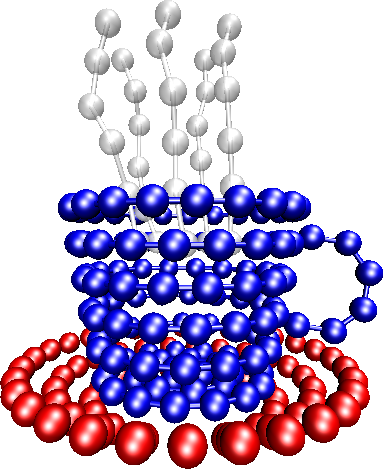
\includegraphics[width=5cm]{logo/transparentbg}
    \end{center}
  }
}


%% Grafikpakete
\usepackage{graphicx}%


\usepackage{verbatim}

% How to diplay ESPResSo commands in flowing text. Larger code segments
% should be put inside boxes.
\newcommand{\EScmd}[1]{\texttt{\textbf{#1}}}

% The code block
%\newcommand{\EScode}[1]{ \parbox{0.95\textwidth}{\texttt{#1}}}
\usepackage{listings} 
\lstset{numbers=left, numberstyle=\tiny, numbersep=5pt, showspaces=false, showstringspaces=false,postbreak=\space, breakindent=5pt, breaklines}
\lstset{language=python, keywordstyle=\color{blue}\bfseries ,emphstyle=\color{green}, commentstyle=\color{red}\itshape }
\lstset{keywordsprefix=setmd}
\lstset{keywords=[6]{thermostat,part,inter,integrate,rescale_velocities,save_sim,writepdb,analyze,uwerr}}

\newtheorem{task}{Task}

\begin{document}

\esptitlehead

\title{Tutorial 1: Lennard-Jones Liquid%
\ifdefined\esversion%
\thanks{For \es \esversion}%
\fi%
}
\subtitle{\es Basics}
\maketitle
\tableofcontents

\section{Introduction}

Welcome to the basic \es{} tutorial!

In this tutorial, you will learn, how to use the \es{} package for your 
research. We will cover the basics of \es, i.e., how to set up and modify a 
physical system, how to run a simulation, and how to load, save and analyze
the produced simulation data.

More advanced features and algorithms available in the \es{} package are 
described in additional tutorials.


\section{Background}

Today's research on Soft Condensed Matter has brought the needs for having a 
flexible, extensible, reliable, and efficient (parallel) molecular simulation 
package. For this reason \es{} (Extensible Simulation Package for Research on 
Soft matter) \cite{esp_url} has been developed at Max Planck Institute for 
Polymer Research, Mainz, and Institute for Computational Physics at the University of Stuttgart in  the group of Prof. Dr. Christian Holm\cite{limbach2006ees,arnold13a}. The Espresso package is probably the most flexible and 
extensible simulation package in the market. It is specially developed for 
coarse-grained molecular dynamics (MD) simulation of polyelectrolytes but not 
necessarily limited to this. It can be used even in simulating granular media 
for example. \es{} has been nominated for the Heinz-Billing-Preis for 
Scientific Computing in 2003 \cite{arnold2003ees}.

\subsection{The Lennard-Jones potential}

A pair of neutral atoms or molecules is subject to two distinct forces in the limit
of large separation and small separation: an attractive force at long ranges (van der
Waals force, or dispersion force) and a repulsive force at short ranges (the result
of overlapping electron orbitals, referred to as Pauli repulsion from Pauli exclusion
principle). The Lennard-Jones potential (also referred to as the L-J potential, 6-12
potential or, less commonly, 12-6 potential) is a simple mathematical model that
represents this behavior. It was proposed in 1924 by John Lennard-Jones. The L-J
potential is of the form
\begin{math}
\label{eq:lj}
    V(r) = 4\epsilon [{({\frac{\sigma}{r}})}^{12} - (\frac{\sigma}{r})^{6}]
\end{math}
where $\epsilon$ is the depth of the potential well and $\sigma$ is the (finite)
distance at which the inter particle potential is zero and $r$ is the distance between
the particles. The $(\frac{1}{r})^{12}$ term describes repulsion and the
$(\frac{1}{r})^{6}$  term describes attraction. The Lennard-Jones potential is an
approximation. The form of the repulsion term has no theoretical justification; the
repulsion force should depend exponentially on the distance, but the repulsion term
of the L-J formula is more convenient due to the ease and efficiency of computing
$r^{12}$ as the square of $r^6$.

\subsection{Units}

Novice users must understand that Espresso has no fixed unit system. The unit 
system is set by the user. Conventionally, reduced units are employed, in other 
words LJ units.
\footnote{If we have charges there is additionally a concept of Bjerrum length, consult Espresso original paper for more details.} 


\section{Python versions}

Espresso can be used both, with python 2 and python 3. In these tutorials, we use python 3 print syntax. If you are on python 2, issue the following command to activate it:
\begin{lstlisting}
from __future__ import print_function
\end{lstlisting}

\section{First steps}\label{sec:espresso}

What is \es{}? It is an extensible, efficient 
Molecular Dynamics package specially powerful on simulating charged systems. 
In depth information about the package can be found in the relevant sources\cite{esp_url,arnold2003ees,limbach2006ees,arnold13a}.

\es consists of two components.
The simulation engine is written in C and C++ for the sake
of computational efficiency. The steering or control
level is interfaced to the kernel via an interpreter 
of the Python scripting languages.

The kernel performs all computationally demanding tasks. Before all,
integration of Newton's equations of motion, including calculation of
energies and forces. It also takes care of internal organization of
data, storing the data about particles, communication between
different processors or cells of the cell-system. 

The scripting interface (Python) is used to setup the system (particles, boundary conditions,
interactions, \dots), control the simulation, run analysis, and store and load results.
The user has at hand the full reliability and functionality of the scripting language.
For instance, it is possible to use the SciPy package for analysis and PyPlot for plotting.
With a certain overhead in efficiency, it can also be
used to reject/accept new configurations in combined MD/MC schemes. In
principle, any parameter which is accessible from the scripting level can be
changed at any moment of runtime. In this way methods like
thermodynamic integration become readily accessible.

\emph{Note: This tutorial assumes that you already have a working \es{}
installation on your system. If this is not the case, please consult the first
chapters of the user's guide for installation instructions.}


Using the pypresso script in the build directory, python simulation scripts can be run conveniently:

\vspace{0,2cm}
\noindent\texttt{./pypresso simulation.py}

\vspace{1cm}\framebox{
    \begin{minipage}{0.95\textwidth} 
        \begin{task} 
             You can check the features, that are compiled in the \es{} core by
             issuing \texttt{print(espressomd.features())} after having imported the 
             \texttt{espressomd} Module. Features can be switched on or off via the \texttt{myconfig.hpp} file. See the chapter on installation in the user's guide.
        \end{task}
    \end{minipage}
}\vspace{1cm}

\begin{pypresso}
import espressomd
print(espressomd.features())
\end{pypresso}


\section{Overview over a simulation script}

Typically, a simulation script consists of the following parts
\begin{itemize}
\item System setup (box geometry, thermodynamic ensemble, integrator parameters)
\item Placing the particles
\item Setup of interactions between particles
\item Warm up (bringing the system into a state suitable for measurements)
\item Integration loop (propagate the system in time and record measurements)
\end{itemize}
In the following sections, it will be shown, how these steps can be taken. Once the basics are covered, we apply them to the simulation of the Lennard-Jones liquid.
Note that only the core elements of the Lennard-Jones simulation script will be covered in this document. The full script can be found in \verb+scripts/lj_tutorial.py+ in the Lennard-Jones tutorial directory.


\subsection{System setup}
The functionality of \es{} for
python is provided via a python module called
\texttt{espressomd}. At the beginning of the simulation script, it has to be imported.
\begin{pypresso}
import espressomd
\end{pypresso}

The next step would be to create an instance of the System class. 
This instance is used as a handle to the simulation system. It can be used to manipulate the
crucial system parameters like the time step and the size of the simulation box (\texttt{time\_step}, and \texttt{box\_l}). At any time, only one instance of the System class can exist.
\begin{pypresso}
system = espressomd.System()
system.time_step = time_step
system.box_l = [box_l_x, box_l_y, box_l_z]
\end{pypresso}

\subsection{Choosing the thermodynamic ensemble, thermostat}
Simulations can be carried out in different thermodynamic ensembles such as NVE (particle Number, Volume, Energy) or NVT (particle Number, Volume, Temperature) as well as NPT-isotropic (particle Number, Pressure, Temperature).
The ensemble is maintained by a thermostat. In this tutorial we use the Langevin thermostat.

In \es{}, the thermostat is set as follows:
{\small\vspace{0,2cm}
\begin{pypresso}
system.thermostat.set_langevin(kT=1.0, gamma=0.5)
\end{pypresso}}\vspace{0,2cm}
\noindent Use a Langevin thermostat (NVT ensemble) with temperature set to 1.0 and damping coefficient to 0.5. Alternatively, the thermostat can be turned off using
{\small\vspace{0,2cm}
\begin{pypresso}
system.thermostat.turn_off()
\end{pypresso}}\vspace{0,2cm}
\noindent This results in an NVE ensemble.


\subsection{Placing and accessing particles}

Particles in the simulation can be accessed via the \texttt{part}-property of the System class. Individual particles are referred to by an integer id, e.g., \texttt{system.part[0]}. It is also possible to use common python iterators and slicing operations to access several particles at once.
\begin{pypresso}
# access position of single particle
print system.part[0].pos

# Iterate over particles
for p in system.part:
    print(p.pos)
    print(p.v)

#Obtain all particle positions
cur_pos = system.part[:].pos
\end{pypresso}
Particles can be grouped into several types, so that, e.g., a binary fluid can be simulated. Particle types are identified by integer ids, which are set via the particles' \texttt{type} attribute. If it is not specified, zero is implied.

Particles are added to the simulation as follows
\begin{pypresso}
system.part.add(id=0, type=0, pos=[x,y,z])
\end{pypresso}\vspace{0,2cm}
Here, \texttt{id} and \texttt{type} can be omitted, in which case an unused particle
id is assigned automatically and type 0 is implied.

Many objects in \es{} have a string representation, and thus can be displayed via python's \texttt{print} method:
\begin{pypresso}
print(system.part[0])
\end{pypresso}\vspace{0,2cm}


\subsection{Setting up non-bonded interactions}

Non-bonded interactions act between all particles of a given combination of particle types.
In this tutorial, we use the Lennard-Jones non-bonded interaction.
The interaction of two particles of type 0 can be setup as follows:
{\small\vspace{0,2cm}
\begin{pypresso}
lj1_eps     = 1.0
lj1_sig     = 1.0
lj1_cut     = 1.12246
lj1_shift   = 0.0
lj1_offset  = 0.0
system.non_bonded_inter[0, 0].lennard_jones.set_params(epsilon=lj_eps, sigma=lj_sig,
cutoff=lj_cut, shift=lj_shift)
\end{pypresso}
}\vspace{0,2cm}


\subsection{Warmup}

In many cases, including this tutorial, particles are initially placed randomly in the simulation box. It is therefore possible that particles overlap, resulting in a huge repulsive force between them. In this case, integrating the equations of motion would not be numerically stable. Hence, it is necessary to remove this overlap.
This is done by limiting the maximum force between two particles, integrating the equations of motion, and increasing the force limit step by step.
This is done as follows
\begin{pypresso}
# Obtain minimum distance between particles
act_min_dist = system.analysis.mindist()
lj_cap=10
while i < warm_n_time and act_min_dist < lj_sigma*0.9 :
    # Set the force cap
    system.non_bonded_inter.set_force_cap(lj_cap)
    lj_cap += 1.0
    # Integrate the equation of motion
    system.integrator.run(100)
    # Obtain minimum distance between particles
    act_min_dist = system.analysis.mindist()

# Disable force cap
system.non_bonded_inter.set_force_cap(0)
\end{pypresso}
In this code fragment, you can also see, how the analysis routines can be used to obtain information about the simulation system, and how to integrate the equation of motion.


\section{Putting it all together: Lennard-Jones liquid simulation}

After we have briefly explained the use of \es{}, we now come to the
Lennard-Jones Liquid Simulation.  Before we explain the script step by step, run the
\texttt{lj\_tutorial.py}  with \texttt{pypresso} to get all generated files.


\subsection{Initialization}

First, we include necessary modules with \lstinline|import|.
{\small\vspace{0,2cm}
\begin{pypresso}
from __future__ import print_function
import espressomd

import os 
import numpy as np

print("""
=======================================================
=                    lj_tutorial.py                   =
=======================================================

Program Information:""")
print(espressomd.features())

\end{pypresso}\vspace{0,2cm}

\subsubsection{System setup}
At first, we must configure the environment and set the needed parameters.
It is good practice to define all simulation parameters as variables in a single location.
{\small\vspace{0,2cm}
\begin{pypresso}
# System parameters
#############################################################
n_part  = 500
density = 0.8442

skin        = 0.1
time_step   = 0.01 
eq_tstep    = 0.001
temperature = 0.728

box_l       = np.power(n_part/density, 1.0/3.0) 

warm_steps  = 100
warm_n_time = 2000
min_dist    = 0.87

# integration
sampling_interval       = 100
equilibration_interval  = 1000

sampling_iterations     = 100
equilibration_iterations= 5 


# Interaction parameters (Lennard Jones)
#############################################################

lj_eps = 1.0
lj_sig = 1.0
lj_cut = 2.5*lj_sig
lj_cap = 5 


# System setup
#############################################################
system              = espressomd.System()

if not os.path.exists('data') :
    os.mkdir('data')

system.time_step    = time_step
system.cell_system.skin         = skin

system.box_l = [box_l, box_l, box_l]

system.non_bonded_inter[0, 0].lennard_jones.set_params(
    epsilon=lj_eps, sigma=lj_sig,
    cutoff=lj_cut, shift="auto")
system.non_bonded_inter.set_force_cap(lj_cap)

print("LJ-parameters:")
print(system.non_bonded_inter[0, 0].lennard_jones.get_params())

# Thermostat
system.thermostat.set_langevin(kT=temperature, gamma=1.0)
\end{pypresso}


\subsection{Particles}
The particles are initially placed randomly in the simulation box

\begin{pypresso}
# Particle setup
#############################################################

volume = box_l * box_l * box_l

for i in range(n_part):
    system.part.add(id=i, pos=np.random.random(3) * system.box_l)
\end{pypresso}}\vspace{0,2cm}

   \vspace{1cm}\framebox{\begin{minipage}{0.95\textwidth} 
   \begin{task}    
   Study the file \texttt{lj\_tutorial.py}. This system mimics the case 
   study 4 of section 4, in the book \cite{frenkel02b}. How can one define 
   truncated-shifted potential in \texttt{lj\_tutorial.py}? ( keep in mind 
   that Espresso has already a factor of 4 at shifted part with cut off 
   $r_{c}=2.5$)
    \[ U(r)= 4 \epsilon\left[ \left(\frac{\sigma}{r} \right)^{12} -  \left(\frac{\sigma}{r} \right)^{6} \right] \]
     
     \[ U(r)^{\text{tr-sh}}  =\left\{ \begin{array}{ll}  U(r)-U(r_{c})  &  r_{c} > r \\
     
     0 &   r_{c}  < r \end{array} \right. \]
     
  (To find the solution look at line 26. Look at picture \ref{pic:lennard-jones} to see a plot of the potential )

   \end{task}

\end{minipage}}\vspace{1cm}

\begin{figure}[ht]
\begin{center}
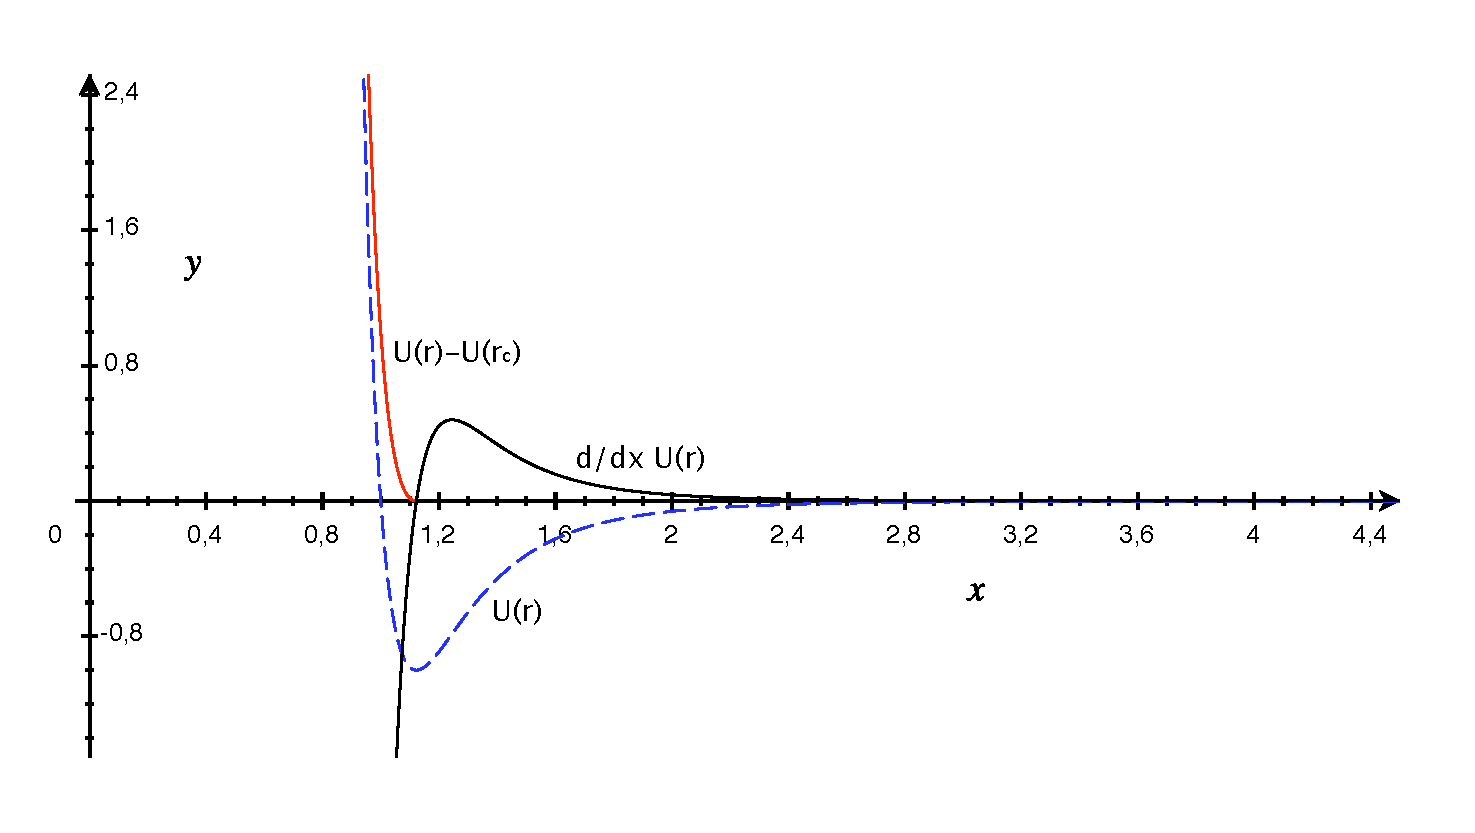
\includegraphics[width=12cm]{figures/lennard-jones-potential.pdf}
%\caption{Lennard Jones Potential - \newline ttt}
\caption[long text]{Lennard-Jones Potential with
  $\epsilon=1$ and radius $\sigma=1$. If you use a large cutoff such as
  $2.5\sigma$, the potential is practically zero at the cutoff. The
  red curve indicates the Weeks-Chandler-Andersen potential, which
  is obtained from the Lennard-Jones potential by cutting it off in
  its minimum at $r_c=\sqrt[6]{2}$ and shifting it up.}
\label{pic:lennard-jones}
\end{center}
\end{figure}


\subsection{Removing the overlap between particles (warmup)}

This removes the overlap between the randomly placed particles, so the system can be integrated in a stable fashion.
\begin{pypresso}
#############################################################
#  Warmup Integration                                       #
#############################################################

print("""
Start warmup integration:
At maximum {} times {} steps
Stop if minimal distance is larger than {}
""".strip().format(warm_n_time, warm_steps, min_dist))

i = 0
act_min_dist = system.analysis.mindist()
while i < warm_n_time and act_min_dist < min_dist :
    system.integrator.run(warm_steps)
    act_min_dist = system.analysis.mindist()
    print("run {} at time = {} (LJ cap= {} ) min dist = {}".strip().format(i, system.time, lj_cap, act_min_dist))
    i+=1
    lj_cap += 1.0
    system.non_bonded_inter.set_force_cap(lj_cap)

system.non_bonded_inter.set_force_cap(0)
\end{pypresso}


\subsection{Integrating the equations of motion, taking measurements}
\noindent At this point, we have set the necessary environment and warmed up our system. As a last
step before starting the actual simulation, we now open the files which we want to output data to
during the simulation. Then the simulation is started.

\begin{pypresso}
# Record energy versus time
en_fp   = open('data/energy.dat', 'w')

# Record radial distribution function
rdf_fp  = open('data/rdf.dat', 'w')

en_fp.write("#\n#\n#\n# Time\ttotal energy\tkinetic energy\tlennard jones energy\ttemperature\n")



# Data arrays for simple error estimation
etotal = np.zeros((sampling_iterations,))

# analyzing the radial distribution function
# setting the parameters for the rdf
r_bins = 50
r_min  = 0.0
r_max  = system.box_l[0]/2.0

avg_rdf=np.zeros((r_bins,))
\end{pypresso}}\vspace{0,2cm}

In the \texttt{energy.dat} file we print out the values for kinetic
and potential energies, temperature obtained with the analysis method 
\lstinline|system.analysis.energy()|. See the code in the snippet above, which
contains the main sampling loop of the script.

\noindent \texttt{kinetic temperature} here refers to the measured temperature
obtained from kinetic energy and the number of degrees of freedom in the system. It
should fluctuate around the preset temperature of the thermostat.

Now, the equations of motion are integrated, and measurements are taken. The radial distribution function is averaged over several measurements, to reduce noise.
\begin{pypresso}
for i in range(1, sampling_iterations + 1):
    system.integrator.run(sampling_interval)
    energies = system.analysis.energy()

    r, rdf = system.analysis.rdf(rdf_type="rdf", type_list_a=[0], type_list_b=[0], r_min=r_min, r_max=r_max, r_bins=r_bins)
    avg_rdf+= rdf/sampling_iterations

    kinetic_temperature = energies['ideal']/( 1.5 * n_part)

    en_fp.write("%f\t%1.5e\t%1.5e\t%1.5e\t%1.5e\n" % (system.time, energies['total'], energies['ideal'], energies['total'] - energies['ideal'], kinetic_temperature))
\end{pypresso}

Finally, the results are saved.
\begin{pypresso}
print("\nMain sampling done\n")

# calculate the variance of the total energy using scipys statistic operations
error_total_energy=np.sqrt(etotal.var())/np.sqrt(sampling_iterations)

en_fp.write("#mean_energy energy_error %1.5e %1.5e\n" % (etotal.mean(), error_total_energy) )

# write out the radial distribution data
for i in range(r_bins):
    rdf_fp.write("%1.5e %1.5e\n" % (r[i], avg_rdf[i]))


en_fp.close()
rdf_fp.close()
\end{pypresso}
The radial distribution function, saved here, (rdf) describes the distribution of particles around
the center of a fixed particle, as a function of the particle-particle distance. This of course assumes
that the particle distribution is isotropic around the particles.
From the rdf, one can see whether the system is in a liquid or crystal state.
For the Lennard-Jones parameters used here, the system is in a liquid state, and particle interactions are significant, as can be seen from the fact that correlations are still visible at a distance of several diameters.

The rdf is computed on the fly in the current script, the data is then written to
\texttt{data/rdf.dat}.


\begin{figure}[ht]
\begin{center}
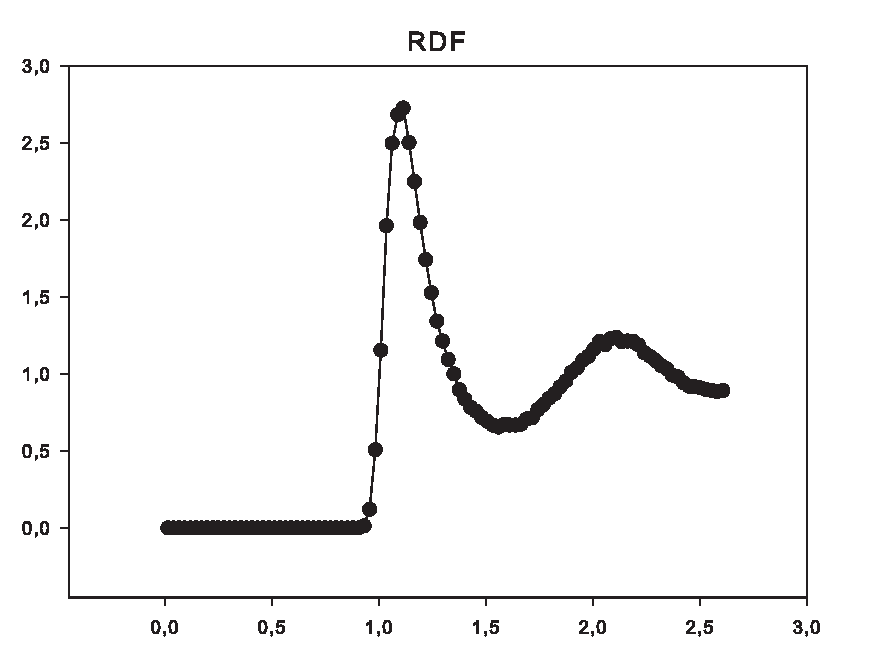
\includegraphics[width=10cm]{figures/rdf}
\label{fig:rdf}
\caption{The rdf.dat plot should be similar to this one}
\end{center}
\end{figure}



\vspace{1cm}\framebox{\begin{minipage}{0.95\textwidth} 
    \begin{task}
      Plot the time evolution of energy and temperature, which are written into the
      \texttt{data} directory in the file \texttt{energy.dat}.
Make sure that the system is in equilibrium by checking that potential, and kinetic energy and calculated current temperature fluctuate around their mean values and do not show a drift.
    \end{task}
  \end{minipage}}\vspace{1cm}

\vspace{1cm}\framebox{\begin{minipage}{0.95\textwidth} 
    \begin{task}
    Re-run the simulation with a density of 0.1 and a Lennard-Jones cutoff of $2^{\frac16}\sigma$. Compare the radial distribution function. Now, the correlations at longer distances are gone, as you are simulating a dilute system with purely repulsive particles. 
    \end{task}
  \end{minipage}}\vspace{1cm}

\subsection{Simple Error Estimation on Time Series Data}
A simple way to estimate the error of an observable is to use the common standard
deviation ($\sqrt{\sigma}$) and the standard error of the mean (SE) for $N$
\emph{uncorrelated} samples:
\begin{align}
    \sigma  &= \langle x^2 - \langle x\rangle^2 \rangle \\
    SE      &= \sqrt{\frac{\sigma}{N}}
    \label{eq:variance}
\end{align}

\begin{pypresso}
# Data arrays for simple error estimation
etotal = np.zeros((sampling_iterations,))
for i in range(1, sampling_iterations + 1):
    energies = system.analysis.energy()

    etotal[i-1] = energies['total']

# calculate the variance of the total energy and total pressure using scipys statistic operations
error_total_energy=np.sqrt(etotal.var())/np.sqrt(sampling_iterations)
\end{pypresso}

\newpage
\section{Exercise: Binary Lennard-Jones Liquid}

%In \es{} it is possible to simulate particles of various sizes, meaning different
%values of the Lennard-Jones parameter $\sigma$. For this purpose there are different mixing
%rules that define how particles of different size and different ``affinity'', Lennard-Jones $\epsilon$ interact. The most commonly used mixing rules are the
%Lorentz-Berthelot rules:
%\begin{align}
%	\sigma_{ij}		& = \frac{\sigma_{ii} + \sigma_{jj}}{2} \\
%	\epsilon_{ij}	& = \sqrt{\epsilon_{ii} \epsilon_{jj}} \,.
%\end{align}
%Here $\sigma_{ii}$ and $\epsilon_{ii}$ are the Lennard-Jones parameters for the
%interactions among particles of type $i$, and $\sigma_{ij}$ and
%$\epsilon_{ij}$ the parameters for interactions between the two species $i$ and $j$.
%
A two-component Lennard Jones liquid can be simulated by placing particles of two types (0 and 1) into the system. 
Depending on the Lennard-Jones parameters, the two components either mix or separate.


\vspace{1cm}\framebox{
    \begin{minipage}{0.95\textwidth} 
        \begin{task}
            \mbox{} 
            \begin{itemize}
            \item Edit the \texttt{lj\_tutorial.py} file such that half of the particles are placed with \texttt{type=1}. Type 0 is implied for the remaining particles
            \item Specify Lennard-Jones interactions for interactions of type 0 particles with other type 0 particles, of type 1 particles with other type 1 particles, and of type 0 particles with type 1 particles (set parameters for \texttt{system.non\_bonded\_inter[i,j].lennard\_jones} where \texttt{i,j} can be \texttt{0,0}, \texttt{1,1}, and \texttt{0,1}).
            Use the same Lennard-Jones parameters for interactions within a component, but use a different \texttt{lj\_cut\_mixed} parameter for the cutoff in the Lennard-Jones interaction between particles of type 0 and particles of type 1. Set this parameter to $2^{\frac16}\sigma$ to get de-mixing or to $2.5\sigma$ to get mixing between the two components. 
            \item Record the radial distribution functions separately for particles of type 0 around particles of type 0, of type 1 around particles of type 1, and finally for particles of type 0 around particles of type 1. This can be done by changing the \texttt{type\_list} arguments of the \texttt{system.analysis.rdf()} command. You can record all three radial distribution functions in a single simulation. It is also possible to write them as several columns into a single file.
            \item Plot the radial distribution functions for all three combinations of particle types. The mixed case will differ significantly, depending on your choice of \texttt{lj\_cut\_mixed}. Explain these differences.
            \end{itemize}

            If you need a hint, look at the \texttt{two-component.py} script in your build directory under \texttt{doc/tutorials/python/01-lennard\_jones/}. Run \texttt{two-component-visualization.py} to see a visualization.
        \end{task}
    \end{minipage}
}\vspace{1cm}


\section{Exercise: Measuring the particles' mean square displacement}

In this task, you will measure the particles' mean square displacement,
\begin{equation}
\mathrm{msd}(t) =\langle (x(t_0+t) -x(t_0))^2\rangle,
\end{equation}
using a concept called ``observables and correlators``.
An observable is an object which takes a measurement on the system. It can depend on parameters, such as the ids of the particles to be considered, which are specified, when the observable is instanced.
\begin{pypresso}
from espressomd.observables import *
part_pos=ParticlePositions(ids=(0,1,2,3))
\end{pypresso}
A correlator is an object which takes results from observables at different times during the simulation, and using a correlation operation, calculates relationships between the observables' values at times $t$ and $t+\delta t$. This can be, e.g., a mean square displacement (expectation value of the square distance a particle has travelled in a certain time) or a velocity autocorrelation (expectation value of the product of the particles' velocities at different time intervals). A correlator for the mean square displacement is instanced as follows
\begin{pypresso}
from espressomd.correlators import *

# The correlator works with the part_pos observable. Here, no second 
# observableis needed

# For short time spans, we record in linear time distances
# for larger time spans, we record in larger and larger steps.
# Use 10 linear measurements 10 time steps apart, each.

# The "square_distance_component_wise" correlation operation tells
# the correlator how to calculate a result from the measurements of the 
# observables at different times

corr=Correlator(obs1=part_pos,
                tau_lin=10,dt=10*time_step,
                tau_max=10000*time_step,
                corr_operation="square_distance_componentwise")
\end{pypresso}
Espresso holds a list of correlators to be automatically updated during integration. The correlator is added to this list as follows
\begin{pypresso}
system.auto_update_correlators.add(corr)
\end{pypresso}
Now the equations of motions can be integrated. This has to be done for a time significantly longer than \texttt{tau\_max}, to obtain good results.
Finally, the results can be obtained as follows
\begin{pypresso}
# The 1st column contains the time, the 2nd column the number of 
# measurements, and the remaining columns the mean square displacement
# for each particle and each Cartesian component
corr.finalize()
result=corr.result()
\end{pypresso}

\vspace{1cm}\framebox{
    \begin{minipage}{0.95\textwidth} 
        \begin{task}
            \mbox{} 
            Record the mean square displacement versus time for a Lennard-Jones liquid. Study its dependence on the density and on the friction parameter ($\gamma$) of the Langevin thermostat.
            \begin{itemize}
            \item Setup up and equilibrate the Lennard Jones liquid as explained in this tutorial
            \item Setup an observable for the particle positions of all particles in the system
            \item Set up a Correlator which records the square distance of the particles for different time intervals. Add it to the list of correlators to be updated automatically.
            \item Integrate the equations of motion
            \item Obtain the results from the correlator, average over all particles and all Cartesian coordinates (column three and above) and write the result to a file
            \item Plot the result
            \end{itemize}

            If you need a hint, look at \texttt{msd.py} in your build directory under \texttt{doc/tutorials/python/01\_lennard-jones/}.
        \end{task}
    \end{minipage}
}\vspace{1cm}


%The velocity autocorrelation function (VACF) is an averaged time dependent correlation function of all particles' 
%velocities. 
%
%\vspace{1cm}\framebox{\begin{minipage}{0.95\textwidth} 
%     \begin{task}  
%      The VACF $C(t)$ can 
%      be computed directly: $ C(t) = \langle {\mathbf v}_{i} (0) {\mathbf v}_{i} (t)
%      \rangle$  which can be estimated by $ C(t) = \frac {1} {N} \sum_{i=0}^{N}
%      {\mathbf v}_{i} (0) {\mathbf v}_{i} (t) $ where $N$ is the number of particles.
%        
%        Try to add this to \texttt{lj\_tutorial.py} by using the functionality of
%        numpy and python.
%     \end{task}
%
%\end{minipage}}
%\vspace{1cm}
%%\marginpar{Script anpassen, sodass kleineres dt, um bessere Aufl\"osung zwischen 0...50 zu erhalten}
%
%\begin{figure}[ht]
%\begin{center}
%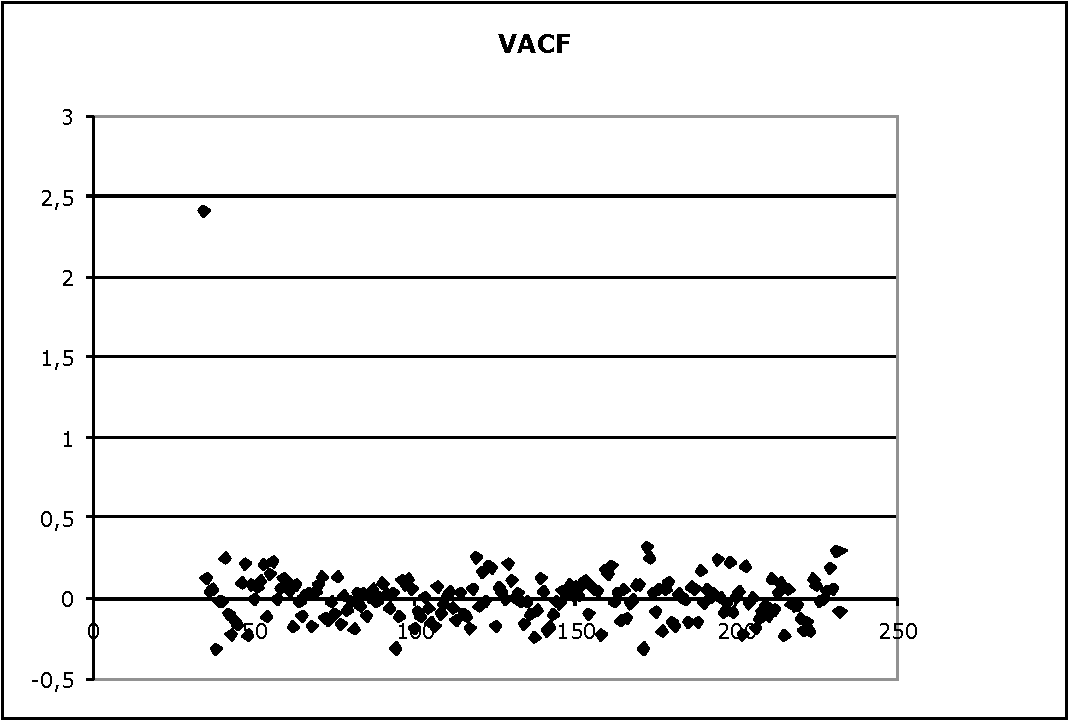
\includegraphics[width=10cm]{figures/vacf}
%\label{fig:vacf}
%\caption{The vacf.dat plot should be similar to this one}
%\end{center}
%\end{figure}
%
%\noindent We can see when time is larger than 50 the particles have already 'forgot' about their initial
%velocities. Sampling more in the time interval [0;50] will show the decay of VACF there.
%
%\newpage

\bibliographystyle{unsrt}
\bibliography{refs}
\end{document}
